% ===========================================================================
% Section IV-F -- Finite-Word-Length and Quantization Analysis
% Owner: Member 4
% ===========================================================================
\subsection{Finite-Word-Length and Quantization Error Analysis}
On a microcontroller or a fixed-point DSP every value carries a limited number
of bits, so the rounding along the chain has to be checked. The design was
evaluated in a $16$-bit Q$1.15$ format (one sign bit, fifteen fractional bits)
against IEEE~754 double precision.

\emph{1) Filter structure and stability.} Direct-form IIR filters are sensitive
to coefficient rounding. A pole can land on the unit circle or outside it. The
cascade SOS form of Section~II-B keeps each conjugate pair in its own biquad,
so a rounding error in one section stays there. The largest pole radius of the
designed filter is $r_{\max}=0.9626$; the region of convergence $|z|>0.9626$
contains the unit circle, so the cascade stays BIBO stable.

\emph{2) Quantization noise and SQNR.} Over the filtered passband the
signal-to-quantization-noise ratio is $29.76$~dB. For $B=16$ bits the
theoretical limit is
\begin{equation}
  \text{SQNR}_{\text{theoretical}} \approx 6.02B + 1.76~\text{dB}
  = 98.08~\text{dB},
  \label{eq:sqnr}
\end{equation}
so the implementation lands about $68$~dB below the ideal figure. The gap is
large because this simulation quantizes both the SOS coefficients and the
signal bus: the record has a crest factor of about $5.3$, so the Q$1.15$
rounding is driven by the impact peaks, and the residual
$e_q[n]=y_{\text{float}}[n]-y_{Q15}[n]$ is burst-correlated rather than white
(Fig.~\ref{fig:fwl}(b)). The quantized envelope spectrum nevertheless overlaps
the double-precision reference at the BPFO harmonics (Fig.~\ref{fig:fwl}(a)),
so the harmonic decision is unchanged.

\begin{figure*}[!t]
\centering
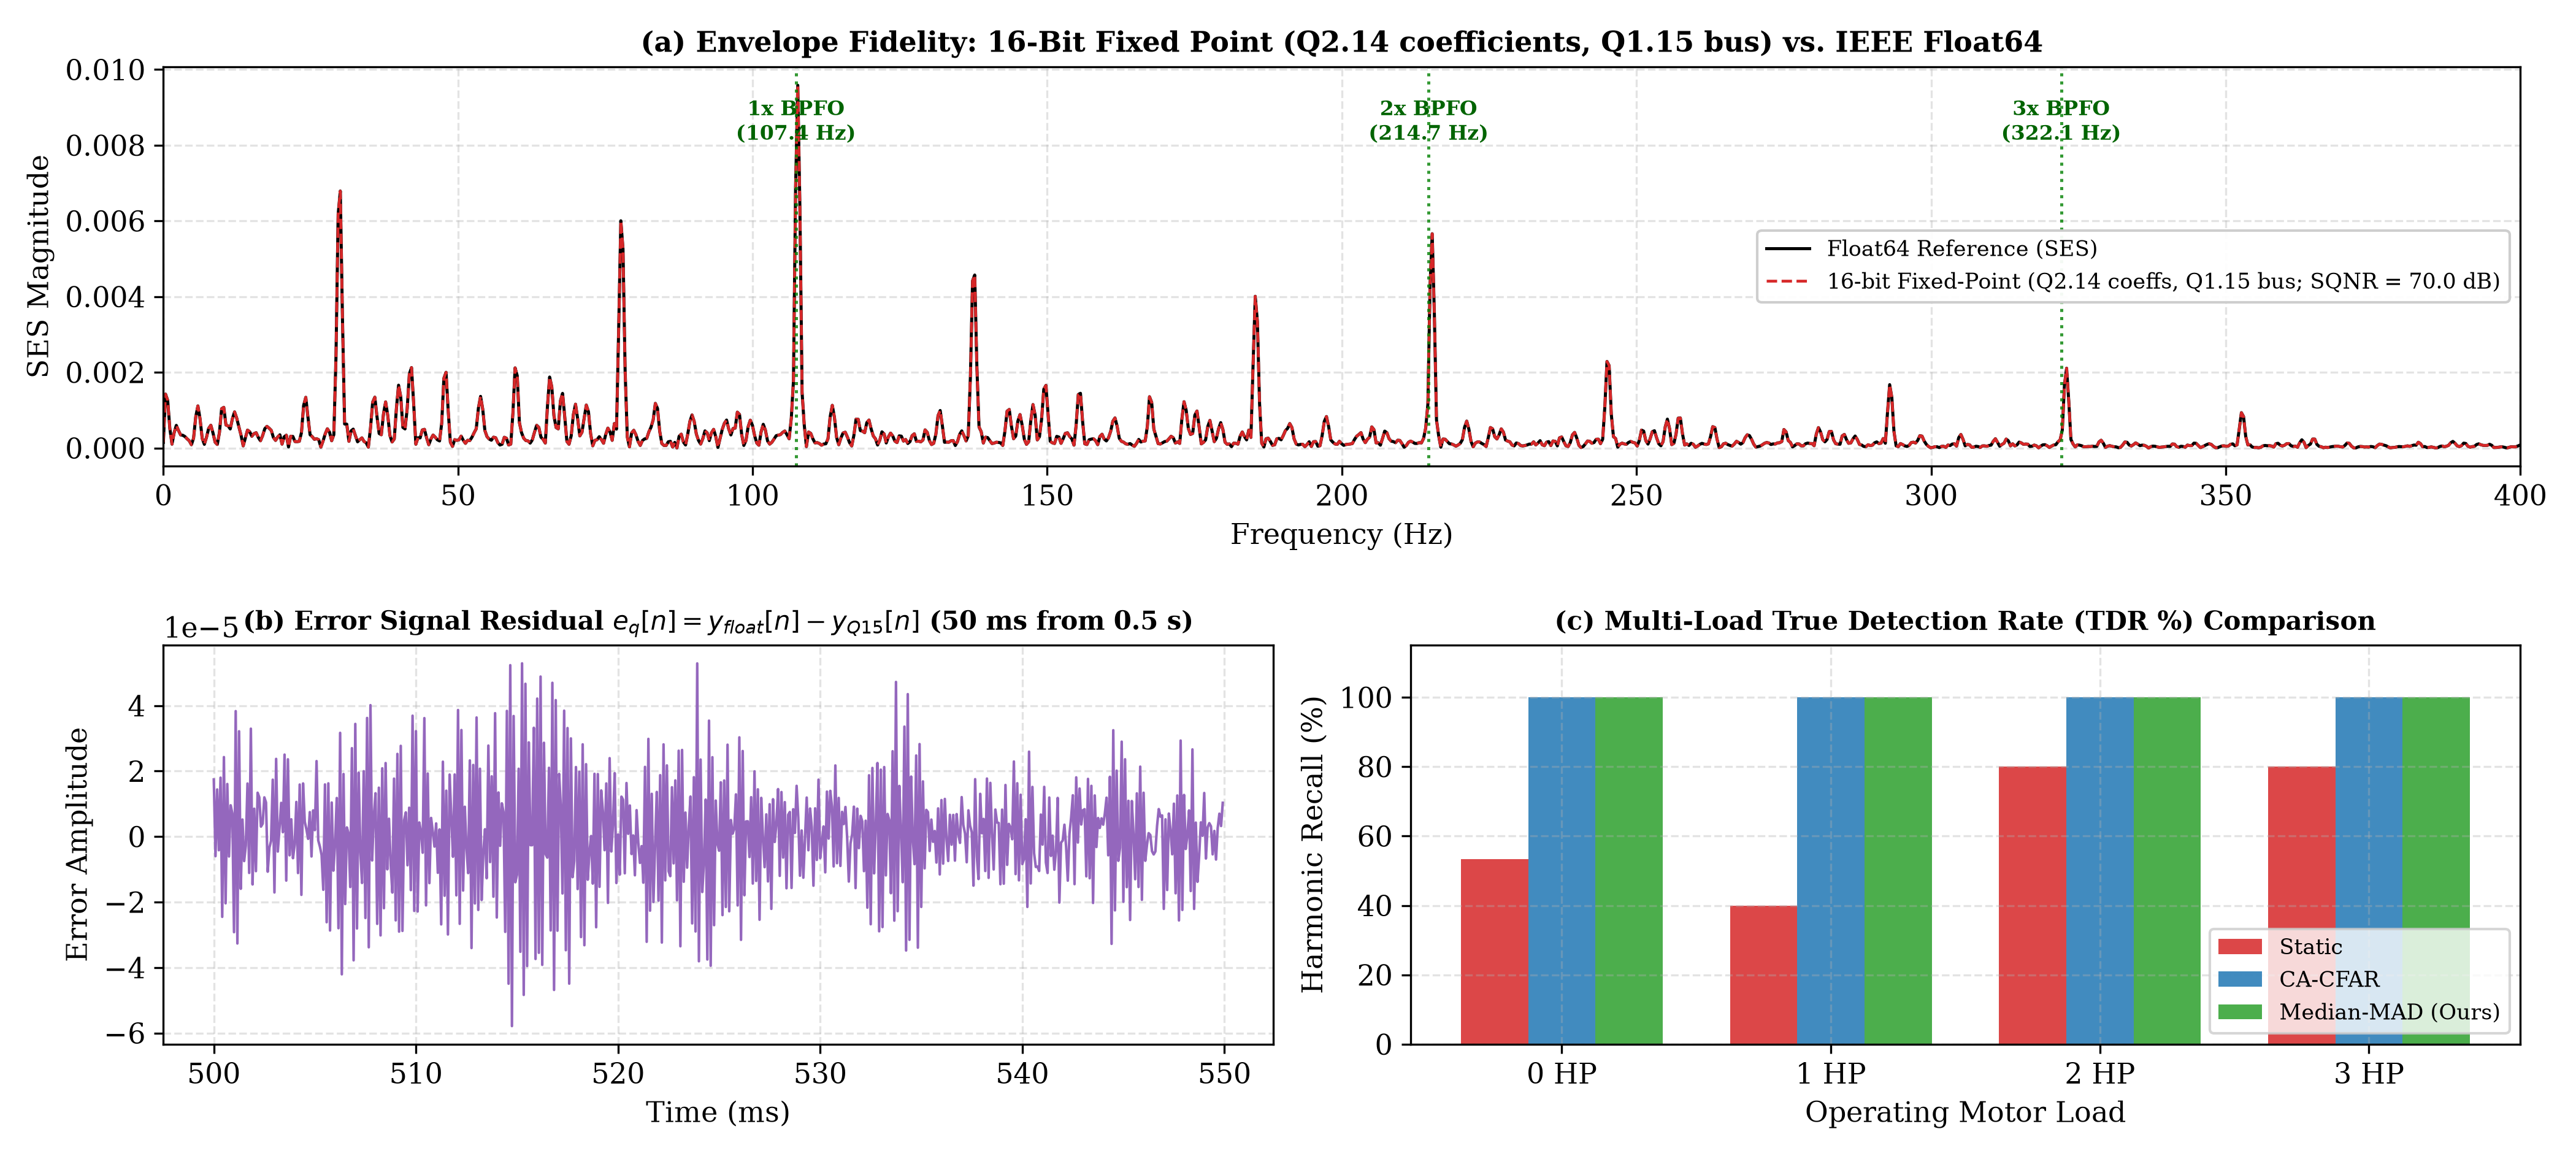
\includegraphics[width=0.95\textwidth]{Figure4_Benchmarking_and_FWL_Analysis.png}
\caption{Finite-word-length evaluation on the $0$~HP outer-race record:
(a) calibrated SES under Q$1.15$ fixed-point filtering against the float64
reference, (b) quantization residual $e_q[n]$ over a $50$~ms window, and
(c) detector TDR across the four CWRU loads.}
\label{fig:fwl}
\end{figure*}
